%%%%%%%%%%%%%%%%%%%%%%%%%%%%%%%%%%%%%%%%%%%%%%
%                insertmeeting
% 1) Title (something creative & funny?)
% 2) Date (MM/DD/YYYY)
% 3) Location (ex. Hagerty High School)
% 4) People/Committees Present 
% 5) Picture 
% 6) Start Time & Stop Time (ex. 12:30AM to 4:30PM)
%%%%%%%%%%%%%%%%%%%%%%%%%%%%%%%%%%%%%%%%%%%%%%
\insertmeeting 
	{Merry-Go-Round} 
	{09/28/21}
	{Hagerty High School}
	{Clayton, Jensen, Nathan, Ritam}
	{Images/RobotPics/robot.jpg}
	{2:30 - 4:30}
	
\subsection*{Hardware}
\noindent\hfil\rule{\textwidth}{.4pt}\hfil
\subsubsection*{Goals}
\begin{itemize}
    \item Continue discussing drivetrain
    \item Prototype carousel mechanism
  

\end{itemize} 

\noindent\hfil\rule{\textwidth}{.4pt}\hfil

\subsubsection*{Accomplishments}
Today we started off the meeting by testing out our idea for the carousel. During the reveal, the carousel stuck out as a very simple and easy to complete task to almost every member, making it a prime subject for our first mechanism. We made it our goal to make a prototype for the carousel to see if our idea will work. Our idea is to attach a wheel to a motor that we can put up against the carousell , spinning the ducks off the platform. Building the prototype proved as simple as we had expected, and we soon had attached a REV grip wheel to a REV core hex motor, hooking it all up to a REV hub so we could control it. When we held the motor up to the carousel, it spun just as we had expected (image 1). Because of the speed of the core hex motor, the duck didn’t fall off of the carousel even at maximum speed. This made us question how much faster we could go. To test out this question, we swapped the core hex motor for a HD hex motor with a 20:1 planetary gearbox. Attaching the wheel in the exact same way, we once again held the mechanism up to the carousel. This time, at the motor’s max speed, the duck flew off (image 2). This means that if we use the faster HD hex motor and slow the speed down slightly in software, we will be able to move at the fastest speed without the duck falling off using the controller, we were able to get the speed pretty fast without making the duck fall off (image 3). 
Another strategy we have for ensuring the duck doesn’t fall off of the carousel takes advantage of the mathematical properties of linear and angular velocity. When we put the duck closer to the center of the carousel, its linear velocity, or how far the duck is actually moving, is lower, meaning the centrifugal force on the duck is lower. When this force is lower, there is less of a chance of the duck flying off the carousel. Usually, if you decrease the velocity, it will take longer for something to go the same distance, but because the carousel is rotating, putting the duck closer to the center does not change the angular velocity, or how many rotations the duck is moving in a certain amount of time. By moving the duck closer to the center, we decrease the linear velocity and the forces applied to the duck, but the angular velocity remains unchanged, meaning it won’t cost us any time. A mathematical proof is shown below: (image 4)

Moving on to the drivetrain, over the weekend, several teams uploaded robot in 3 days (Ri3D) robot reveals. By watching the simple prototyping of some other teams, we saw that formal drivetrains like mecanum and tank can still go over the barrier poles, as long as the wheels hit the poles first. This might mean that a completely new drivetrain design won’t be necessary and we can use a similar basic design that we’ve been adjusting and changing to fit new needs every year. We still plan on creating the lighter, 4 wheeled tank drive prototype once the parts arrive, but to keep our options open, we are also going to test our designs from previous years as well.
The first design that we are going to test is the mecanum drivetrain that we designed and built over the summer. We are happy to know that this drivetrain might still have a use for us during this season, but because we didn’t think it would go over the barriers, we left it in a partial state of disrepair. When the game reveal came out, we were in the middle of adding spacers to the wheels and replacing all of the shafts, but we never finished doing all of this. Because we have a newfound use for the drivetrain, we still need to rebuild it. Using a small chop saw in our room, we cut a steel shaft into the correct length for our wheels (image 5). Once the shafts were cut, we pressed them into the pulleys, added the spacers into the wheels and put the rest of the drivetrain back together. At this point in the meeting, we ran out of time, but we still plan on testing the mecanum drive, and our 6- wheel tank drive.


\begin{figure}[ht]
\centering
\begin{minipage}[b]{.50\textwidth}
  \centering
  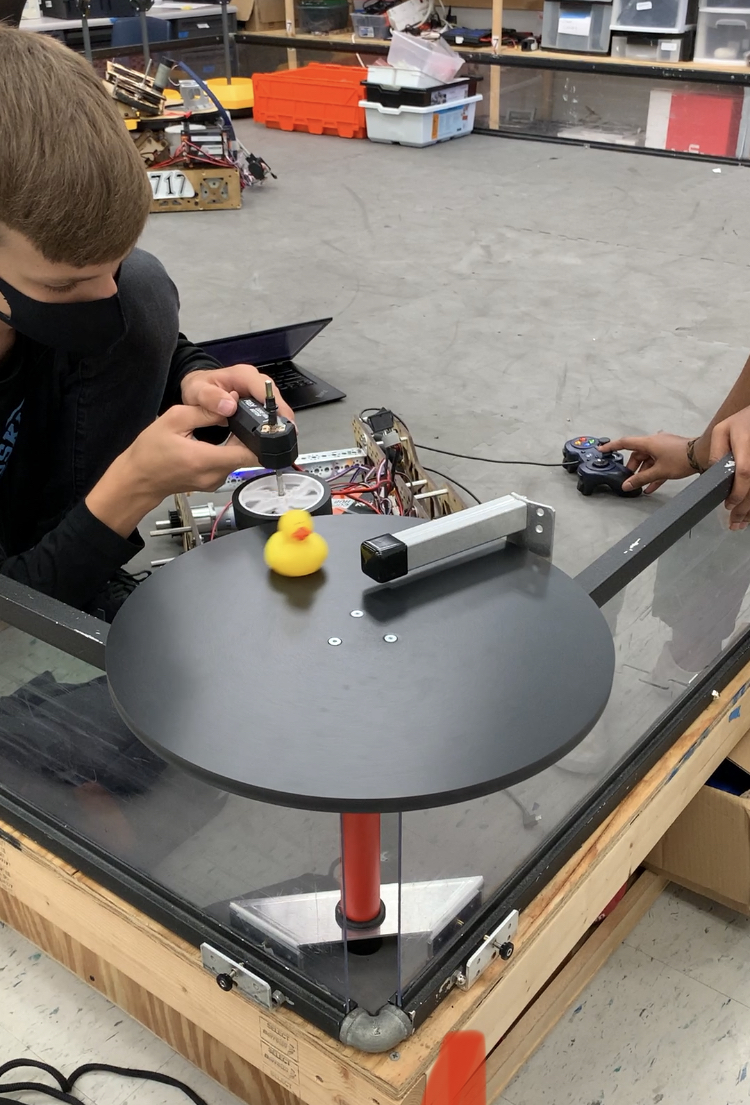
\includegraphics[width=0.8\textwidth]{Meetings/September/09-28-21/9-28-21_Hardware_Image1 - Nathan Forrer.jpg}
  \caption{Using a traction wheel to prototype a carousel spinner.}
  \label{fig:pic1}
\end{minipage}%
\hfill%
\begin{minipage}[b]{.50\textwidth}
  \centering
  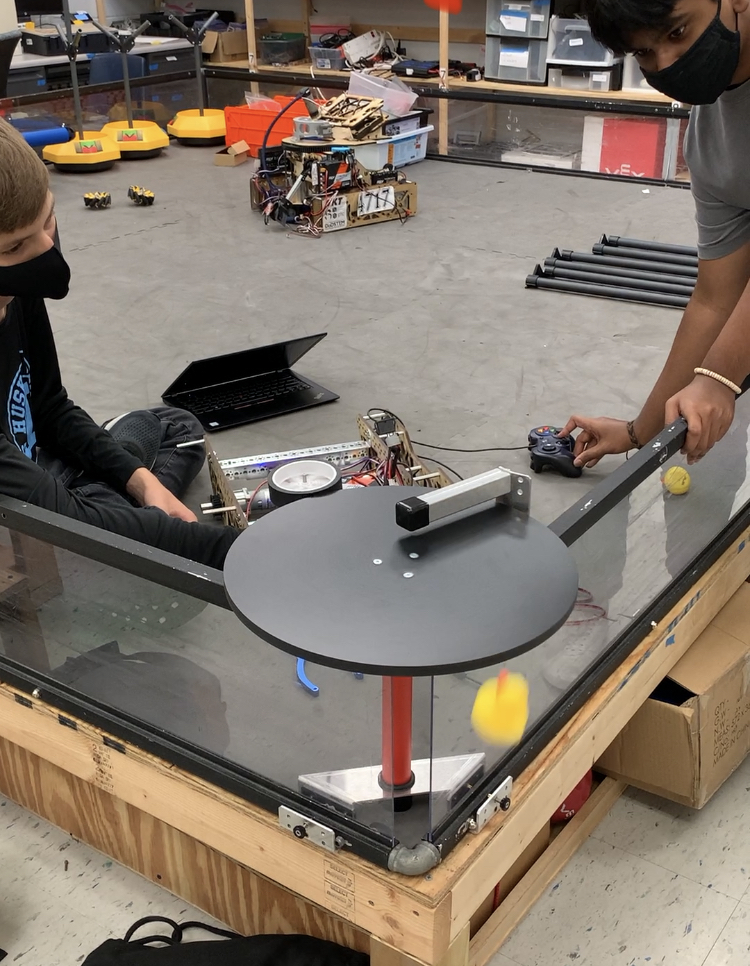
\includegraphics[width=0.8\textwidth]{Meetings/September/09-28-21/9-28-21_Hardware_Image2 - Nathan Forrer.jpg}
  \caption{Another angle of our prototype.}
  \label{fig:pic2}
\end{minipage}
\end{figure}

\begin{figure}[ht]
\centering
\begin{minipage}[b]{.50\textwidth}
  \centering
  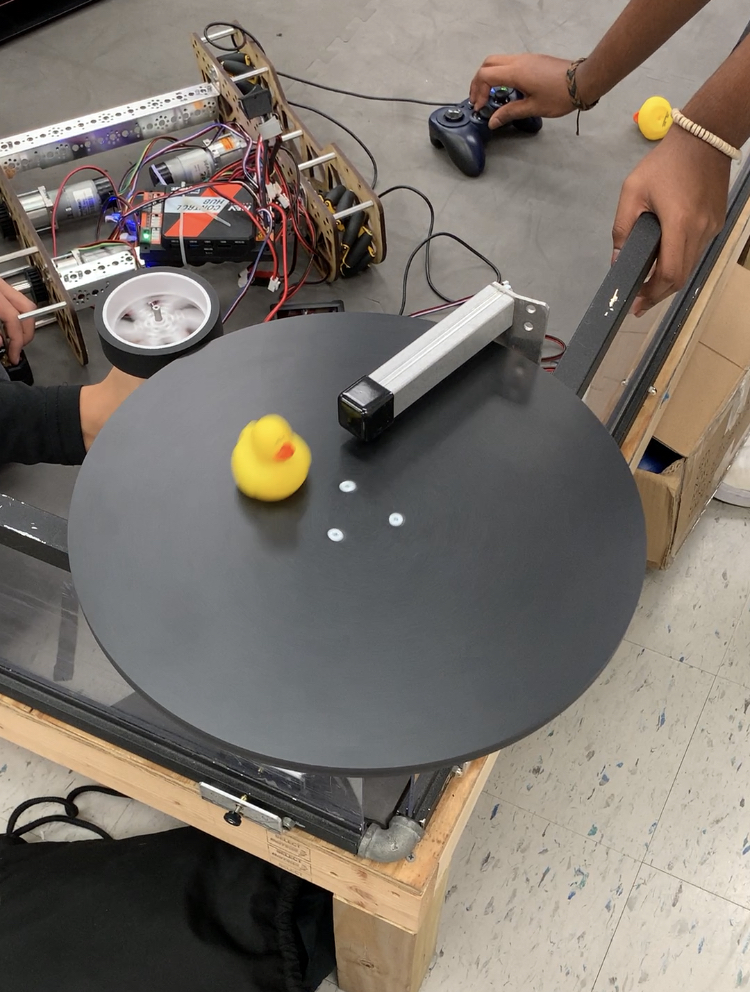
\includegraphics[width=0.8\textwidth]{Meetings/September/09-28-21/9-28-21_Hardware_Image3 - Nathan Forrer.jpg}
  \caption{The prototype in action.}
  \label{fig:pic3}
\end{minipage}%
\hfill%
\begin{minipage}[b]{.50\textwidth}
  \centering
  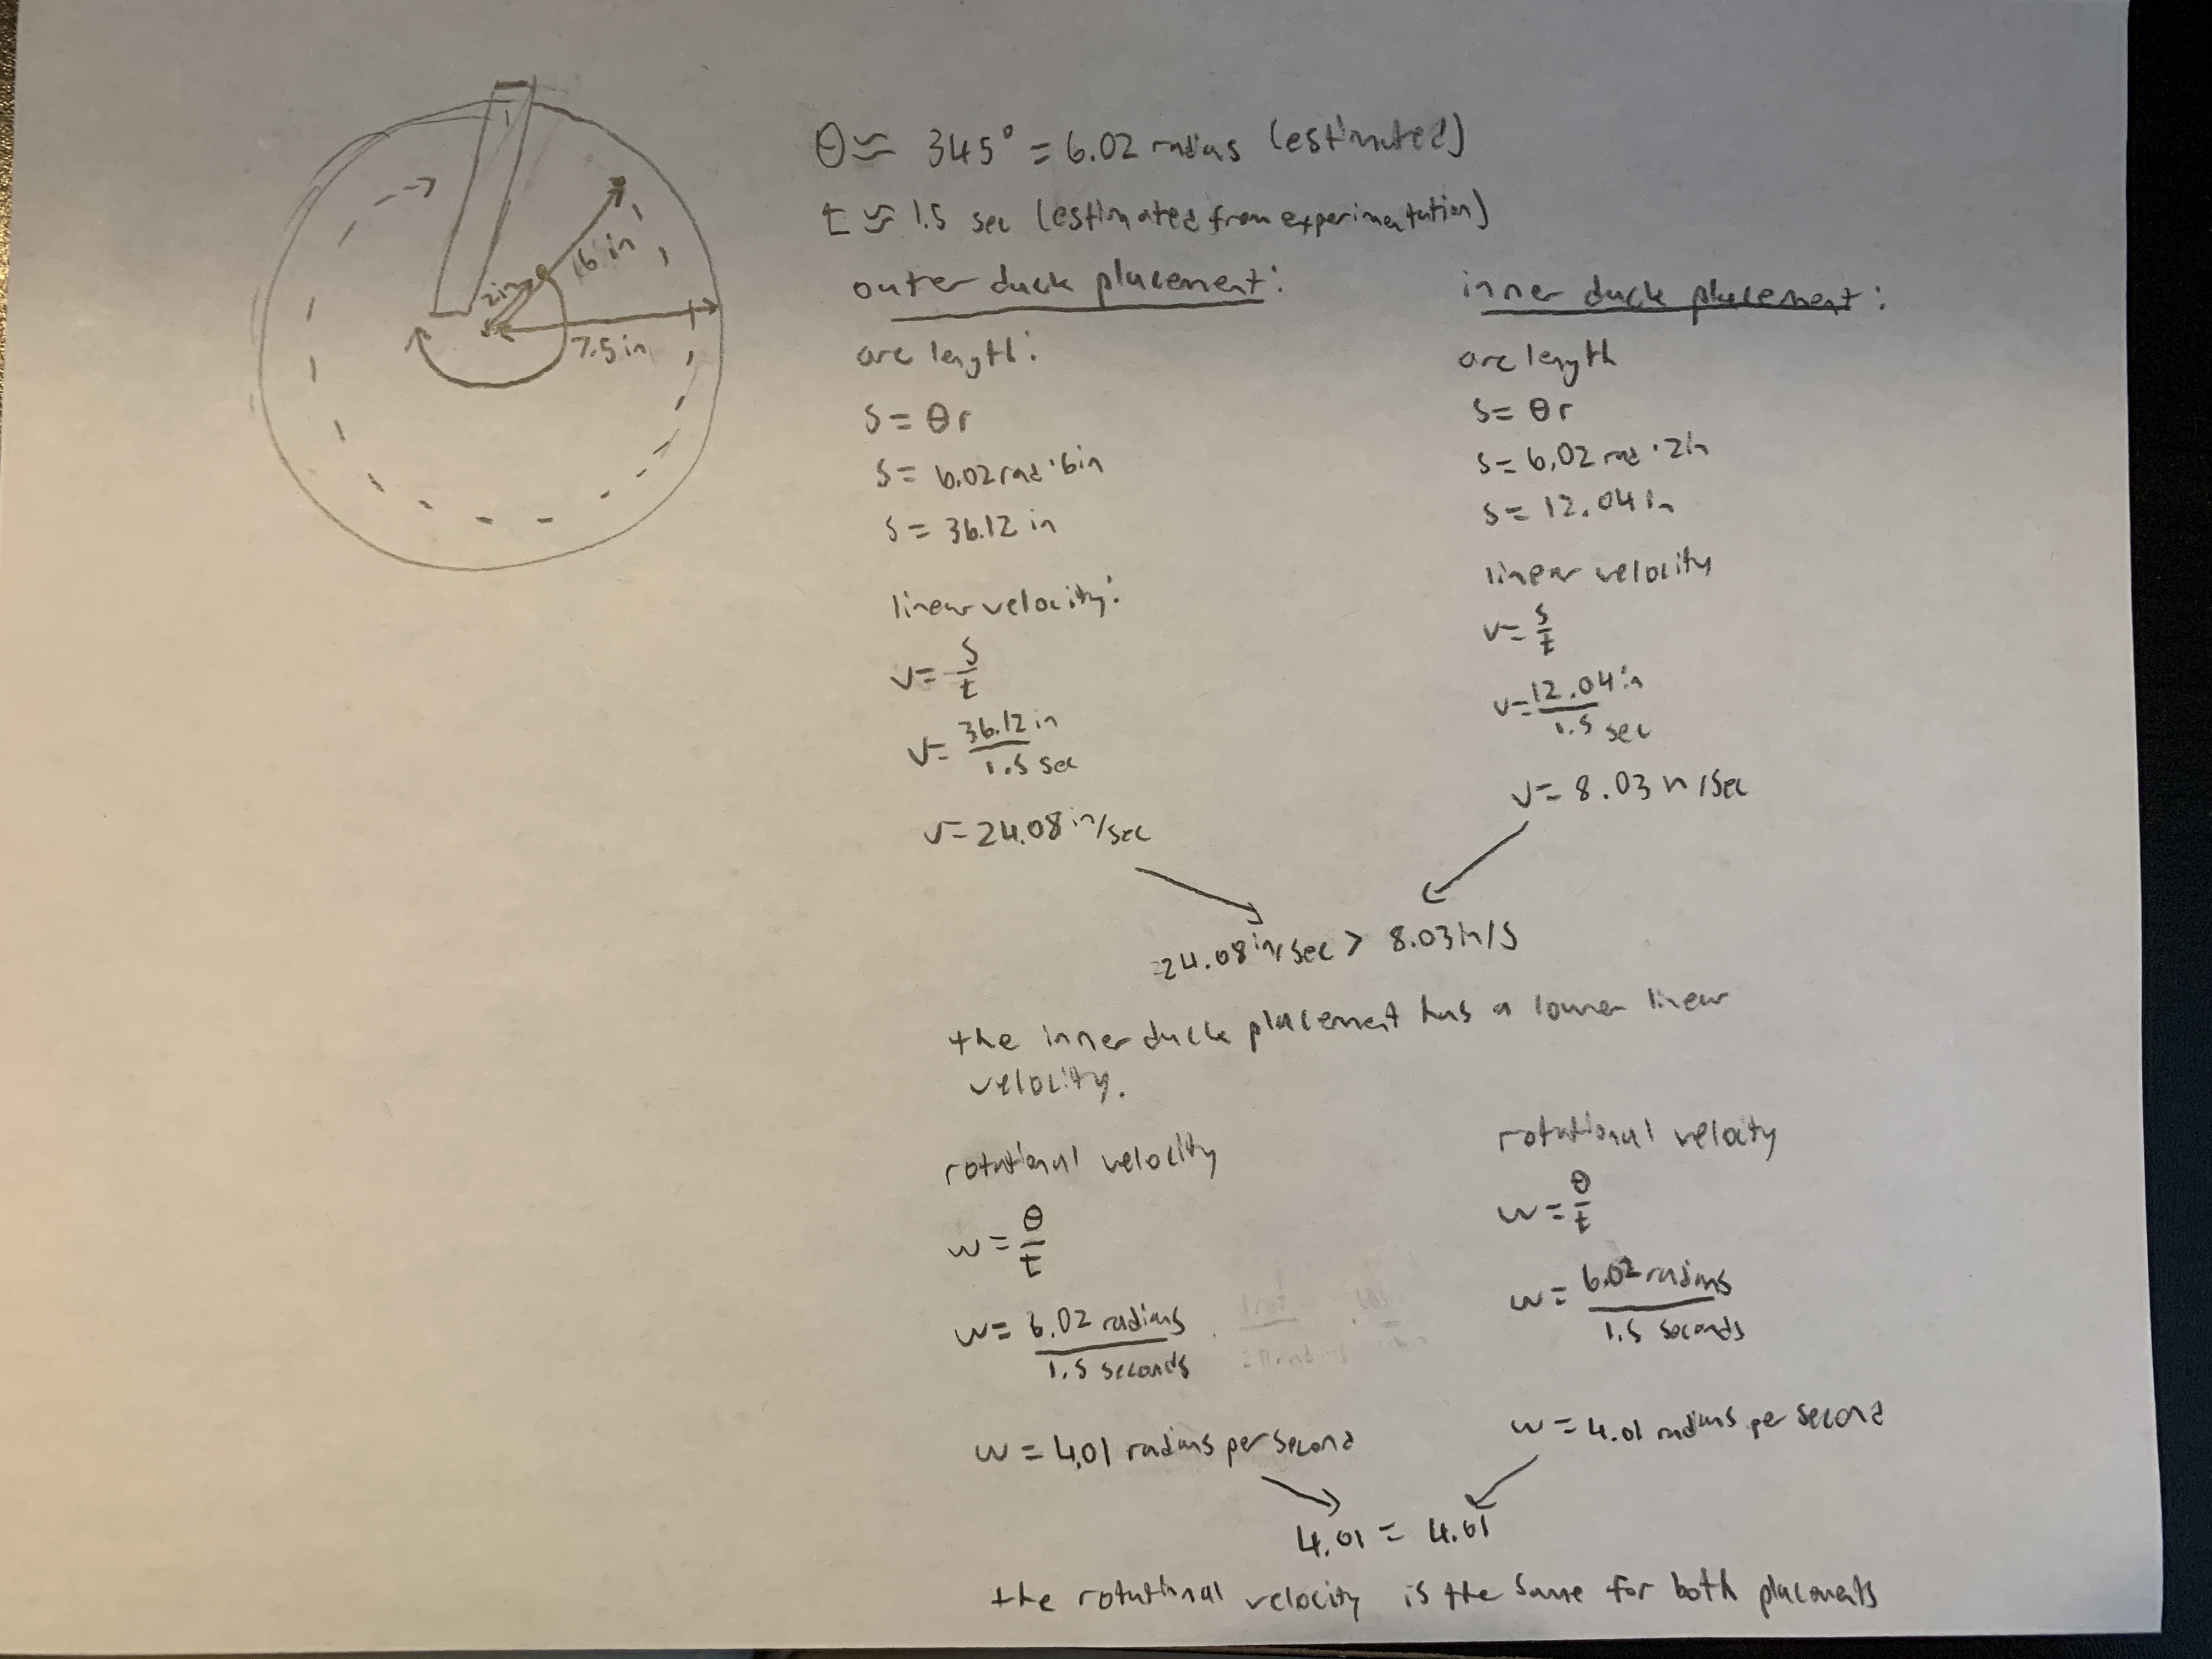
\includegraphics[width=0.8\textwidth]{Meetings/September/09-28-21/9-28-21_Hardware_Image4 - Nathan Forrer.jpg}
  \caption{The calculations used in designing a carousel spinner mechanism.}
  \label{fig:pic4}
\end{minipage}
\end{figure}

\begin{figure}[htp]
\centering
  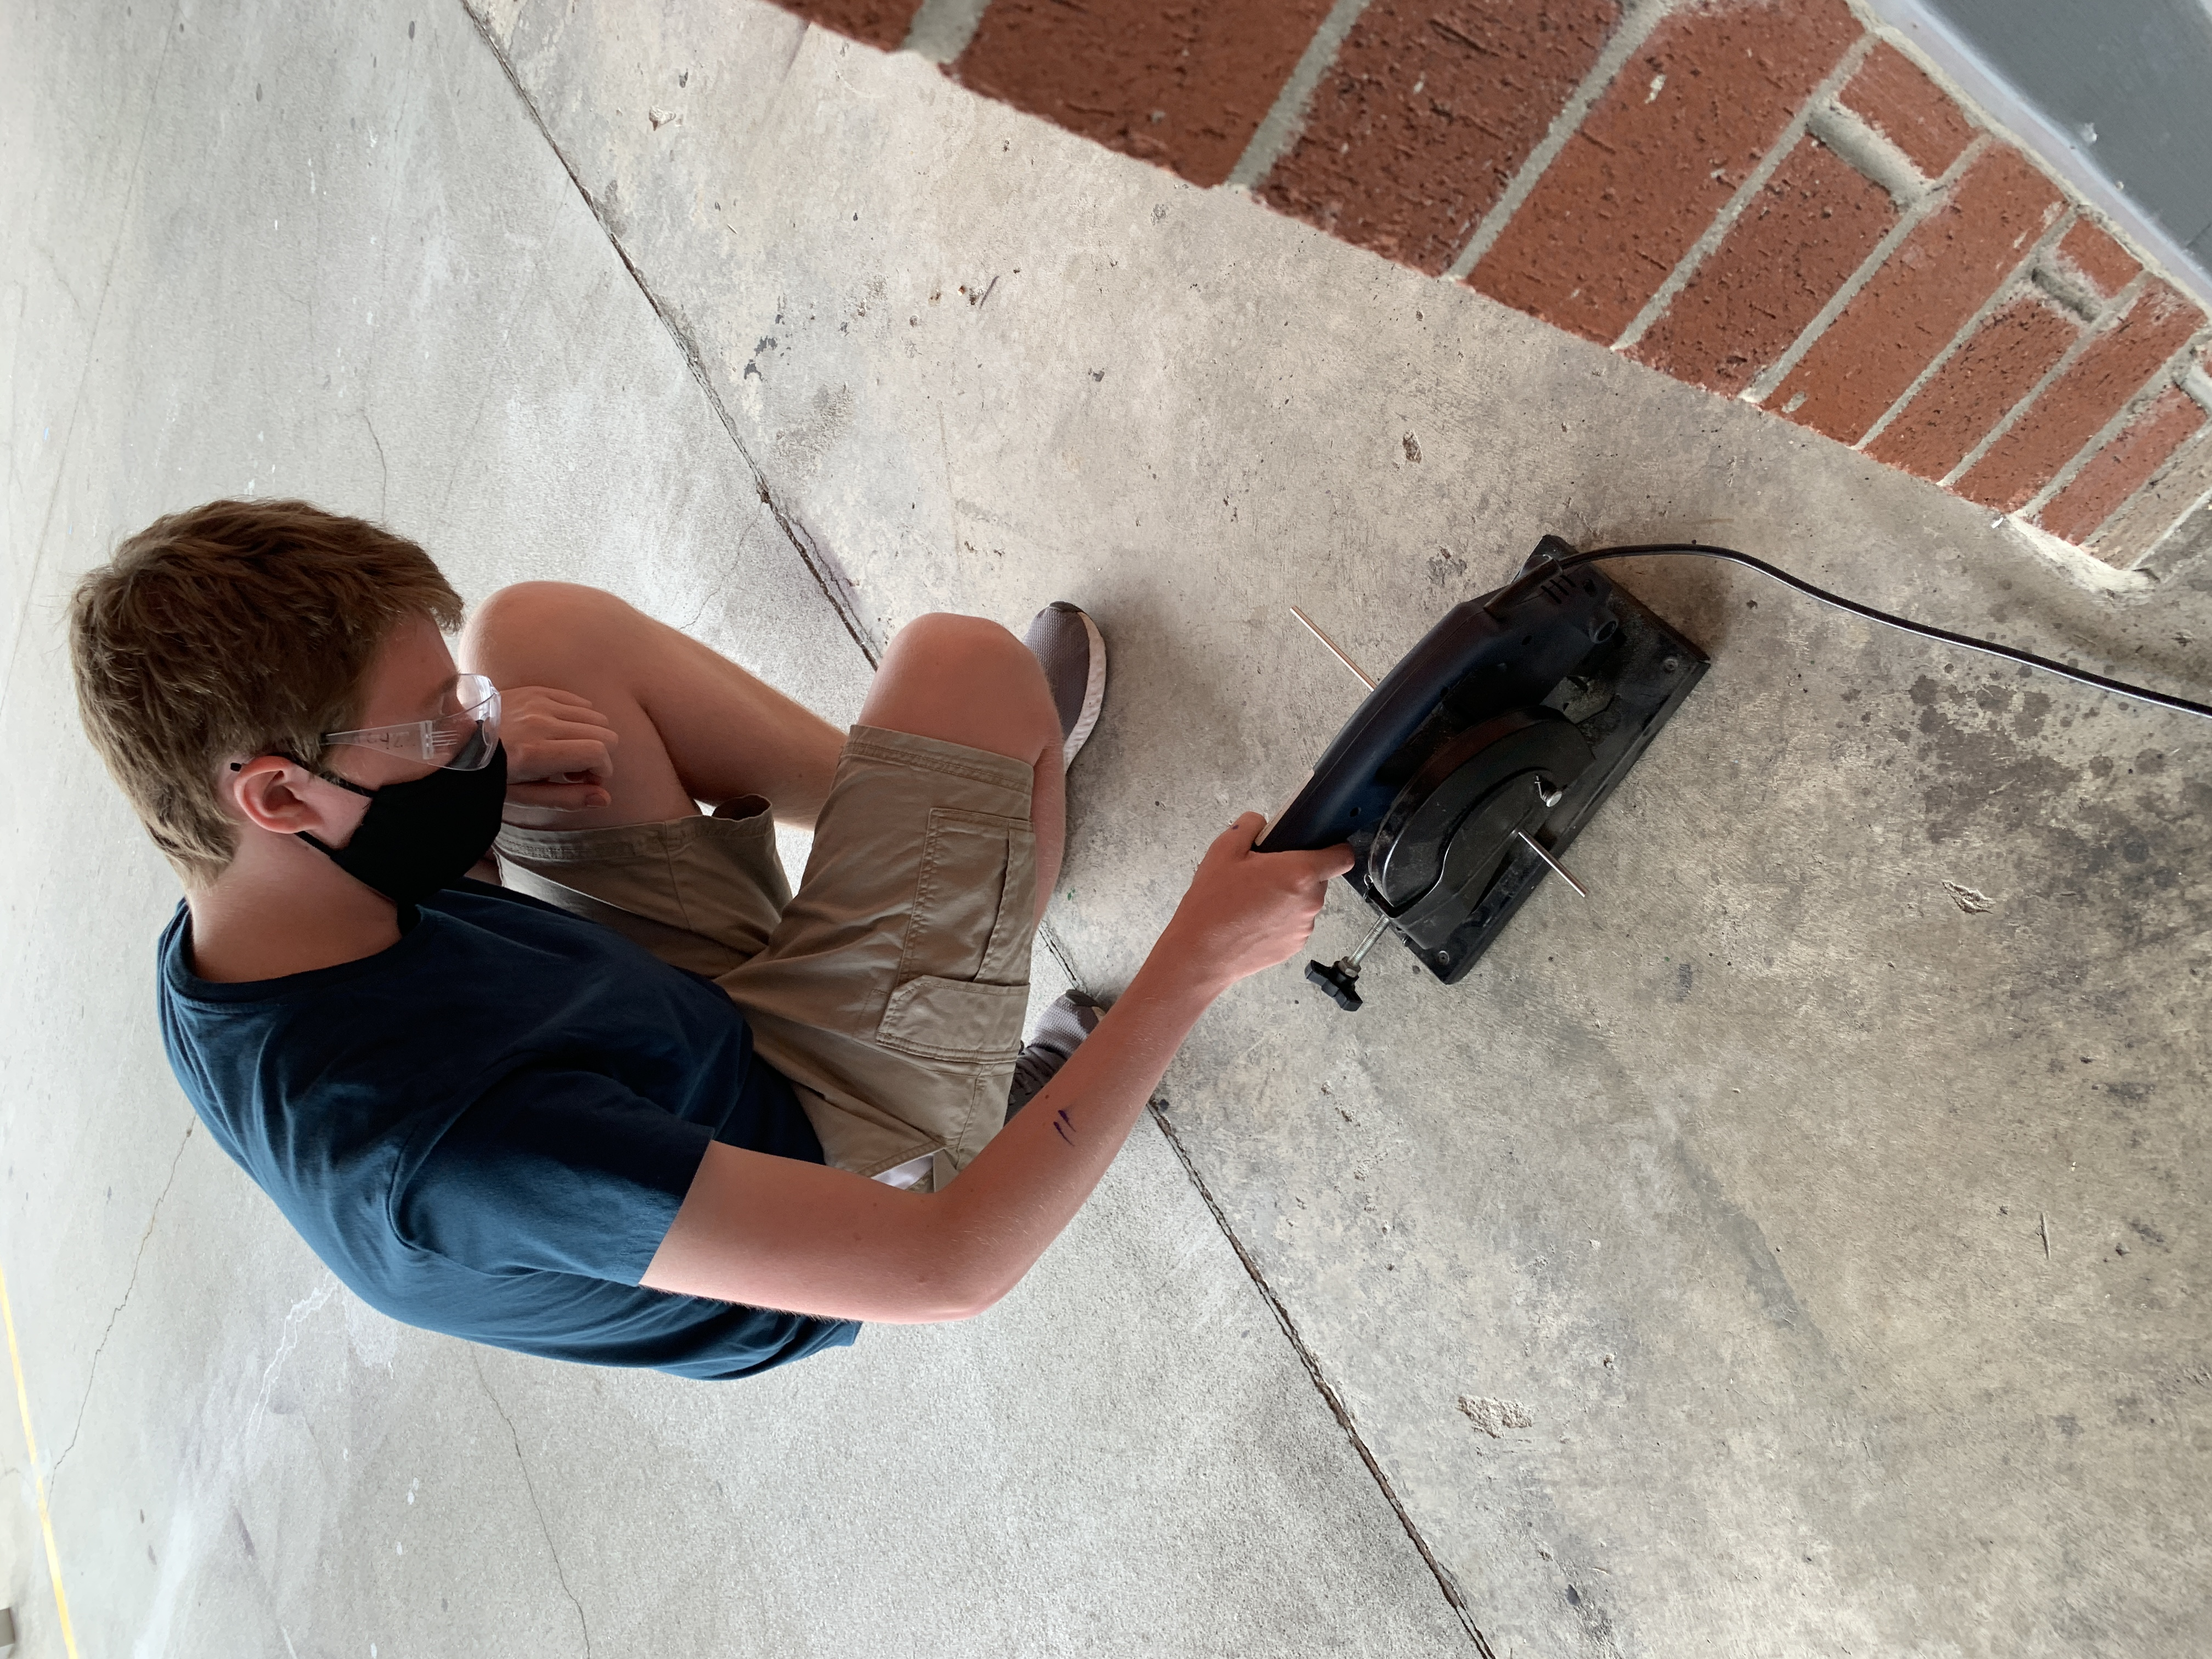
\includegraphics[width=0.8\textwidth]{Meetings/September/09-28-21/9-28-21_Hardware_Image5 - Nathan Forrer.jpg}
  \caption{Nathan cutting a hex shaft using a chopsaw.}
  \label{fig:pic5}
\end{figure}